% Template ACM. O modo nonacm remove os dados de publicação da ACM.
\documentclass[sigconf,nonacm]{acmart}

% Permite quebrar nomes de modelos e evita estouros de margem.
\renewcommand{\texttt}[1]{\nolinkurl{#1}}
\setlength{\emergencystretch}{2em}

% Notação dos contrastes (decisão 0016): o primeiro índice entra com sinal positivo.
\newcommand{\Dcb}{D_{\mathrm{code},\mathrm{base}}}
\newcommand{\Dic}{D_{\mathrm{instr},\mathrm{code}}}
\newcommand{\Dib}{D_{\mathrm{instr},\mathrm{base}}}

% Espaço entre referências (evita Overfull na última página).
\setlength{\bibsep}{1pt plus 1pt}

% Diagrama do experimento nos anexos; [H] fixa tabelas e figuras dos anexos depois do texto.
\usepackage{float}
\usepackage{tikz}
\usetikzlibrary{arrows.meta,positioning}

% Numeração das páginas (o sigconf a omite por padrão).
\settopmatter{printfolios=true}
\begin{document}

\title{Code Specialization, Instruction Tuning, and Atoms of Confusion}
\subtitle{Comparing Perplexity Across General-Purpose Base, Code-Specialized Base, and Instruct Models} 

\author{Camila Nicola Dias Santana, João Marcos de Sousa Rezende, Matheus Botelho Menezes dos Santos, and Samuel Souza Silva}
\affiliation{\institution{Universidade Federal de Minas Gerais}\city{Belo Horizonte}\country{Brazil}}
\renewcommand{\shortauthors}{Santana, Rezende, Santos, and Silva}

\begin{abstract}
Abdelsalam et al.\ showed that code language models assign higher perplexity to atoms of confusion, in line with neural signals of human confusion.
We reproduce their study and compare eight trios of related base, code, and instruct checkpoints from five families on Java and C snippets.
Recomputed statistics match the authors' result files, and all six published models remain significant when pairs are clustered by base pair.
General-purpose base models already show the effect in Java. The evidence on code specialization and instruction tuning is mixed, with contrasts in both directions.
In Java, perplexity correlates with the human FRP on confusing snippets in all 24 models (Spearman $\rho = 0.32$--$0.53$), while no interval excludes zero on clean snippets.
In C, the confusion effect is smaller and five of its 24 intervals include zero.
\end{abstract}

\maketitle

\section{Problem and Motivation}
Software, like natural language, is repetitive and predictable~\cite{hindle2012}, and, as word surprisal predicts reading difficulty, more surprising versions of meaning-equivalent snippets took programmers longer to answer correctly~\cite{casalnuovo2020}.
Atoms of confusion, small patterns that cause programmers to misread code, were identified in C~\cite{gopstein2017} and later studied in Java~\cite{langhout2021}; more than 30\% of the Java files in the Android Open Source Project contain at least one~\cite{tabosa2024}.
Bergum et al.\ showed that atoms elicit a late frontal positivity in fixation-related potentials (FRP), like unexpected but plausible words~\cite{bergum2025}, and Abdelsalam et al.\ found that LLM perplexity on the same snippets, especially in the area of interest (AOI) that contains the atom, correlates with this response~\cite{abdelsalam2026}.
They evaluated mostly code models (their package includes one general-purpose model, Llama 3.2 3B); we reproduce their study, compare related base, code, and instruct checkpoints, and extend it to the C snippets of Gopstein et al.

We compare trios of related checkpoints: a general-purpose base model ($B$), its code-specialized version ($C$), and the instruct version of the code model ($I$).
Models in a trio share a lineage and tokenize every snippet identically, but may differ in vocabulary, context length, data and recipe, so differences are associated with, not attributed to, code specialization and instruction tuning.
For each pair, $\ell = \ln(\mathrm{PPL}_{\mathrm{confusing}}) - \ln(\mathrm{PPL}_{\mathrm{clean}})$, and a model's confusion effect is $\Delta = \bar{\ell}$.
Maximum AOI-level perplexity is the exponential of the maximum token surprisal within the AOI. The secondary snippet-level perplexity uses the mean.
We report $\Dcb = \Delta_C - \Delta_B$, $\Dic = \Delta_I - \Delta_C$ and $\Dib = \Delta_I - \Delta_B = \Dcb + \Dic$ on the AOI metric, prespecified before any trio was run.
Nominal 95\% intervals come from a percentile bootstrap (10\,000 resamples, seed 42) over clusters shared by the three models of a trio (24 base pairs in Java, 20 atoms in C).


\section{Experimental Setup}
\paragraph{Models.}
Eight trios from five families (Qwen2.5 3B, 7B and 32B, DeepSeek 7B, Yi 9B, Llama-2 7B and 13B, and Gemma 7B; Appendix~\ref{app:design}), all evaluated on Java and C in fp16, except Qwen2.5 32B (4 bits).
Instruct models score plain snippets, without chat templates; Gemma is reported only with maximum AOI-level perplexity.

\paragraph{Data.}
We use the 72 Java pairs of Bergum et al.~\cite{bergum2025} and the original C dataset~\cite{gopstein2017}, from which they descend~\cite{langhout2021}.
We use all 21 atoms of the authors' package, 15 of them confirmed as confusing by the original study.
The Java AOI was designed with the stimuli and checked in a pilot study; for C we annotated one (Section~\ref{sec:discussion}), and the dead-code atom, which has no clean AOI, is left out of the AOI metric (60 pairs, 20 atoms).

\section{Results}
\paragraph{Reproduction.}
We recomputed RQ1--RQ3 from the published outputs of Qwen2.5-Coder-32B and re-executed \texttt{deepseek-coder-1.3b-base} locally (Apple Silicon, fp16; Appendix~\ref{app:reproduction}).
The four RQ1 tests match the paper at its precision, and all recomputed statistics match the authors' result files. Two results printed in the paper differ from those files (RQ2 clean: $\rho = 0.063$ versus $0.05$; RQ3 overlap, clean: bootstrap mean $0.42$ versus $0.38$, point estimate $0.41$), without changing the original conclusions.
The original tests (Wilcoxon for RQ1, Spearman $p$ values for RQ2), like our reproduction, treat the 72 pairs as independent, although they come from 24 base pairs. With a bootstrap clustered by base pair, all six published models keep intervals above zero for $\Delta$ and for $\rho$ on confusing snippets.
The re-execution has identical tokens and nearly identical statistics ($W = 863$ versus $864$), but only 84.5\% of tokens fall within our prespecified tolerance (99\% required), consistent with numerical noise; the criterion remains unmet.


\begin{figure}[t]
  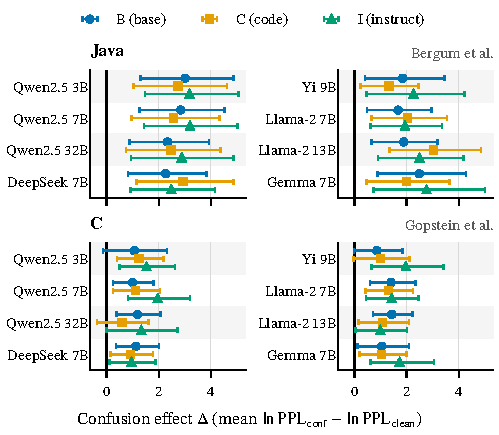
\includegraphics[width=\columnwidth]{../results/extensao/2026-11-11-figuras/delta-aoi_max-grade.pdf}
  \caption{Confusion effect $\Delta$ (maximum AOI-level perplexity) for each base (B), code (C) and instruct (I) model, with nominal 95\% bootstrap intervals; Java above, C below; Qwen2.5 32B in 4 bits.}
  \label{fig:delta}
\end{figure}


\paragraph{Confusion effect.}
In Java, all 24 models assign higher perplexity to the AOI of confusing snippets ($\Delta$ from 1.32 to 3.19, all intervals above zero; Figure~\ref{fig:delta}).
In C, effects are smaller ($\Delta$ from 0.59 to 1.97), and five intervals include zero: Qwen2.5 3B base, Qwen2.5 32B code and instruct, and Yi 9B base and code.




\begin{table}[t]
  \caption{Contrasts between models for maximum AOI-level perplexity, with nominal 95\% bootstrap intervals. Bold: interval excludes zero.}
  \label{tab:extension}
  {\scriptsize\setlength{\tabcolsep}{2.5pt}
\begin{tabular}{lccc}
\toprule
Family & $D_{\mathrm{instr},\mathrm{base}}$ & $D_{\mathrm{code},\mathrm{base}}$ & $D_{\mathrm{instr},\mathrm{code}}$ \\
\midrule
\multicolumn{4}{l}{\textit{Java (Bergum et al.)}} \\
\midrule
Qwen2.5 3B & 0.17 [$-$0.35, 0.69] & $-$0.27 [$-$0.99, 0.36] & 0.44 [$-$0.02, 0.92] \\
Qwen2.5 7B & 0.35 [$-$0.31, 1.08] & $-$0.29 [$-$0.72, 0.14] & \textbf{0.64 [0.01, 1.29]} \\
Qwen2.5 32B (4 bits) & 0.55 [$-$0.20, 1.27] & 0.13 [$-$0.31, 0.62] & 0.41 [$-$0.13, 0.97] \\
DeepSeek 7B & 0.22 [$-$0.26, 0.69] & 0.67 [$-$0.05, 1.36] & $-$0.45 [$-$0.96, 0.03] \\
Yi 9B & 0.42 [$-$0.30, 1.13] & $-$0.53 [$-$1.20, 0.11] & \textbf{0.94 [0.004, 1.92]} \\
Llama-2 7B & 0.27 [$-$0.07, 0.65] & \textbf{0.37 [0.004, 0.78]} & $-$0.10 [$-$0.32, 0.10] \\
Llama-2 13B & 0.61 [$-$0.004, 1.23] & \textbf{1.14 [0.25, 2.06]} & \textbf{$-$0.54 [$-$0.94, $-$0.12]} \\
Gemma 7B & 0.28 [$-$0.51, 1.05] & \textbf{$-$0.50 [$-$0.82, $-$0.21]} & \textbf{0.78 [0.07, 1.50]} \\
\midrule
\multicolumn{4}{l}{\textit{C (Gopstein et al.)}} \\
\midrule
Qwen2.5 3B & 0.47 [$-$0.32, 1.22] & 0.18 [$-$0.48, 0.88] & 0.28 [$-$0.003, 0.58] \\
Qwen2.5 7B & \textbf{0.96 [0.43, 1.52]} & 0.10 [$-$0.23, 0.43] & \textbf{0.86 [0.41, 1.30]} \\
Qwen2.5 32B (4 bits) & 0.15 [$-$0.63, 0.81] & \textbf{$-$0.59 [$-$1.03, $-$0.19]} & \textbf{0.74 [0.19, 1.29]} \\
DeepSeek 7B & $-$0.17 [$-$0.58, 0.25] & $-$0.20 [$-$0.59, 0.20] & 0.03 [$-$0.16, 0.21] \\
Yi 9B & \textbf{1.11 [0.14, 2.05]} & 0.13 [$-$0.50, 0.83] & \textbf{0.98 [0.42, 1.62]} \\
Llama-2 7B & 0.03 [$-$0.38, 0.42] & $-$0.10 [$-$0.51, 0.24] & 0.13 [$-$0.12, 0.36] \\
Llama-2 13B & \textbf{$-$0.44 [$-$0.81, $-$0.09]} & \textbf{$-$0.35 [$-$0.72, $-$0.01]} & $-$0.09 [$-$0.20, 0.03] \\
Gemma 7B & \textbf{0.69 [0.27, 1.16]} & 0.01 [$-$0.25, 0.27] & \textbf{0.68 [0.19, 1.24]} \\
\bottomrule
\end{tabular}}

\end{table}

\paragraph{Correlation with EEG (RQ2).}
In Java, Spearman $\rho$ between maximum AOI-level perplexity and the human FRP ranged from 0.32 to 0.53 on confusing snippets, all intervals above zero, and from $-0.13$ to 0.15 on clean ones, none excluding zero (Table~\ref{tab:app-eeg}).

\paragraph{Contrasts.}
In Java, $\Dib$ is positive in all eight trios, but no interval excludes zero.
Across both languages, $\Dic$ is positive in 12 of 16 trio--language combinations, with eight intervals excluding zero (seven positive, some with lower bounds close to zero, and one negative, Llama-2 13B in Java). Five $\Dcb$ intervals exclude zero, in both directions (Table~\ref{tab:extension}; per-model results in Appendix~\ref{app:results}).

\section{Discussion and Threats to Validity}
\label{sec:discussion}
Because atoms are common in real code~\cite{tabosa2024}, code specialization can change exposure to them in either direction (more code, or quality filtering that removes them). Curation differs across vendors, consistent with $\Dcb$ of opposite signs across families (e.g., Llama-2 13B and Gemma 7B in Java), but we did not measure corpus composition.
With dozens of nominal intervals, some bold entries are expected by chance, and an interval that includes zero is not evidence of no effect.

Every instruct model is built on the code model, so $\Dic$ compares each instruct model with the code model it was tuned from, in a fixed order. Instruction recipes also differ across families.
Instruct models ran without chat templates; for Qwen2.5 3B and DeepSeek 7B, adding the template lowered $\Delta_I$ in 6 of 8 language--metric combinations without reversing its sign, but 5 of the 16 contrasts involving the instruct model, mostly close to zero, changed sign (e.g., $\Dic$ of Qwen2.5 3B in Java, 0.44 to $-0.05$).

The AOI maximum also depends on how many tokens the AOI contains, which varies across versions, languages and tokenizers, so comparisons between families and sizes are descriptive.
Java and C differ at once in language, snippet style and atom categories (C has macro, preprocessor and pointer atoms), so the smaller effects in C are not attributed to the language alone.
The C AOI is an assumption: Gopstein et al.\ validated atoms by error rates on whole snippets, not by region, and our annotation was produced by an LLM under author-defined rules, with examples from 26 pairs checked (four revised rules unchecked). Across three AOI annotations, 12 of the 24 primary C contrasts changed sign or interval status, several of them close to zero.
Four atoms were unconfirmed and two (indentation) left out of the original analysis; restricted to the 15 confirmed atoms (45 pairs), every C $\Delta$ increases and only a near-zero contrast reverses ($\Dcb$ of Gemma 7B), but $\Dib$ and $\Dic$ of Qwen2.5 3B then exclude zero, whereas $\Dib$ and $\Dcb$ of Llama-2 13B no longer do.

The 32B trio ran in 4 bits, which lowered $\Delta$ of \texttt{Qwen2.5-Coder-32B} in Java from 2.75 (published fp16) to 2.47; a common precision within the trio does not ensure that the error cancels in the contrasts.
Each vendor contributes one family, the snippets are short synthetic programs, and there are EEG data only for Java: in C, the link to human confusion remains indirect.

\section{Conclusion}
In Java, maximum AOI-level perplexity already separates confusing from clean code in all eight general-purpose base models, so the alignment with atoms of confusion precedes additional code specialization. Pretraining may already include code, as for Qwen2.5~\cite{qwen25}, and the snippet-level metric rarely shows the effect.
The evidence on instruction tuning and code specialization is mixed: $\Dic$ is often positive but negative for Llama-2 13B, and $\Dcb$ excludes zero in both directions; we find no consistent effect of either stage.

In Java, perplexity is positively associated with the published FRP on confusing snippets in every model; we did not test differences between these correlations. Results in C remain conditional on the AOI annotation and the evaluated atom set.

\section*{AI-Assistance Statement}
The authors designed the reproduction and extension.
AI agents (Claude Opus 5.5, Claude Sonnet 5.5 and GPT-6 Astra) implemented code under the authors' direction and assisted with tests, documentation and drafting.
The AOI annotation of the C dataset was produced in a hybrid process by the authors and two independent AI agents.
The authors validated the code and are responsible for the final text.

\bibliographystyle{ACM-Reference-Format}
\bibliography{references}

% Anexos, em uma coluna e a partir da página seguinte às referências.
\onecolumn
% Anexos do artigo (main.tex), incluídos depois das referências.
\appendix
% Numeração por anexo: Figura A.1, Tabela B.2 etc.
\counterwithin{figure}{section}
\counterwithin{table}{section}
% Sem esticar o espaço vertical (o \flushbottom do template abre vãos entre as tabelas).
\raggedbottom

\section{Experimental Design}
\label{app:design}

Figure~\ref{fig:app-design} summarizes the experiment, Table~\ref{tab:app-models} lists the 24 checkpoints and Table~\ref{tab:app-revisions} the revision of each one.
The reproduction (top row) checks the original analyses before the extension (bottom row) reuses their metric on new models and on the C dataset.
In C, the maximum AOI-level metric uses 60 pairs from 20 atoms (the dead-code atom has no clean AOI), and the snippet-level metric all 63 pairs from 21 atoms; bootstrap clusters follow the atoms of each metric.

\begin{figure}[H]
  \centering
  \begin{tikzpicture}[
      font=\footnotesize,
      box/.style={draw, rounded corners=2pt, align=flush left, inner sep=4pt, text width=#1, minimum height=2.2cm},
      box/.default=3cm,
      lane/.style={font=\footnotesize\bfseries, anchor=west},
      arr/.style={-{Latex[length=2mm]}, thick},
      node distance=4mm]
    % Reproduction
    \node[lane] (rlab) at (0, 0) {Reproduction};
    \node[box=3.4cm, below=1mm of rlab.south west, anchor=north west] (r1)
      {\textbf{Published outputs}\\
       Replication package of Abdelsalam et al.\ (6 models, 72 Java pairs, published FRP)};
    \node[box=3.6cm, right=of r1] (r2)
      {\textbf{Recomputation}\\
       RQ1--RQ3 statistics for Qwen2.5-Coder-32B, compared with the paper and the authors' result files};
    \node[box=3.6cm, right=of r2] (r3)
      {\textbf{Re-execution}\\
       \texttt{deepseek-coder-1.3b-base} in fp16, token by token (tolerance not met);\\
       Qwen2.5-Coder-32B in 4 bits vs.\ published fp16};
    \node[box=3.8cm, right=of r3] (r4)
      {\textbf{Robustness}\\
       Bootstrap clustered by base pair (24 clusters) for RQ1 and RQ2 of the six published models};
    \draw[arr] (r1) -- (r2);
    \draw[arr] (r2) -- (r3);
    \draw[arr] (r3) -- (r4);

    % Extension
    \node[lane, below=5mm of r1.south west, anchor=north west] (elab) {Extension};
    \node[box=3.4cm, below=1mm of elab.south west, anchor=north west] (e1)
      {\textbf{Data}\\
       Java: 72 pairs = 24 base pairs $\times$ 3 versions; AOI designed with the EEG stimuli\\
       C: 63 pairs = 21 atoms $\times$ 3; AOI annotated by us (60 pairs, 20 atoms)};
    \node[box=3.6cm, right=of e1] (e2)
      {\textbf{Models}\\
       8 trios, 5 families (Table~\ref{tab:app-models})\\[2pt]
       $B \xrightarrow{\text{code}} C \xrightarrow{\text{instr.}} I$\\[2pt]
       Plain snippets, no chat template; fp16 (32B trio: 4 bits)};
    \node[box=3.6cm, right=of e2] (e3)
      {\textbf{Metrics}\\
       Per-token log-probabilities\\
       Max.\ AOI-level PPL (primary); snippet-level mean PPL (secondary)\\
       $\ell = \ln \mathrm{PPL}_{\mathrm{conf}} - \ln \mathrm{PPL}_{\mathrm{clean}}$, $\Delta = \bar{\ell}$};
    \node[box=3.8cm, right=of e3] (e4)
      {\textbf{Analyses}\\
       Contrasts $\Dcb$, $\Dic$, $\Dib$\\
       Cluster bootstrap: 10\,000 resamples, seed 42, shared within a trio\\
       RQ2: Spearman $\rho$ with FRP (Java only)};
    \draw[arr] (e1) -- (e2);
    \draw[arr] (e2) -- (e3);
    \draw[arr] (e3) -- (e4);
    \draw[arr, dashed] (r3.south) -- node[right, font=\scriptsize, align=left] {scoring code\\checked in\\re-execution} (e3.north);
  \end{tikzpicture}
  \caption{Structure of the experiment. Top: reproduction of Abdelsalam et al.; bottom: extension to trios of related checkpoints and to the C dataset. The extension reuses the scoring implementation checked in the re-execution; most trios use an equivalent single forward pass per snippet.}
  \label{fig:app-design}
\end{figure}

\begin{table}[H]
  \caption{Checkpoints of the eight trios (Hugging Face identifiers). All trios are evaluated on Java and C.}
  \label{tab:app-models}
  \footnotesize
  \begin{tabular}{llll}
    \toprule
    Trio & Base ($B$) & Code ($C$) & Instruct ($I$) \\
    \midrule
    Qwen2.5 3B & \texttt{Qwen/Qwen2.5-3B} & \texttt{Qwen/Qwen2.5-Coder-3B} & \texttt{Qwen/Qwen2.5-Coder-3B-Instruct} \\
    Qwen2.5 7B & \texttt{Qwen/Qwen2.5-7B} & \texttt{Qwen/Qwen2.5-Coder-7B} & \texttt{Qwen/Qwen2.5-Coder-7B-Instruct} \\
    Qwen2.5 32B (4 bits) & \texttt{mlx-community/Qwen2.5-32B-4bit} & \texttt{mlx-community/Qwen2.5-Coder-32B-4bit} & \texttt{mlx-community/Qwen2.5-Coder-32B-Instruct-4bit} \\
    DeepSeek 7B & \texttt{deepseek-ai/deepseek-llm-7b-base} & \texttt{deepseek-ai/deepseek-coder-7b-base-v1.5} & \texttt{deepseek-ai/deepseek-coder-7b-instruct-v1.5} \\
    Yi 9B & \texttt{01-ai/Yi-9B} & \texttt{01-ai/Yi-Coder-9B} & \texttt{01-ai/Yi-Coder-9B-Chat} \\
    Llama-2 7B & \texttt{meta-llama/Llama-2-7b-hf} & \texttt{meta-llama/CodeLlama-7b-hf} & \texttt{meta-llama/CodeLlama-7b-Instruct-hf} \\
    Llama-2 13B & \texttt{meta-llama/Llama-2-13b-hf} & \texttt{meta-llama/CodeLlama-13b-hf} & \texttt{meta-llama/CodeLlama-13b-Instruct-hf} \\
    Gemma 7B & \texttt{google/gemma-7b} & \texttt{google/codegemma-7b} & \texttt{google/codegemma-7b-it} \\
    \bottomrule
  \end{tabular}
\end{table}

\begin{table}[H]
  \caption{Hugging Face revisions (first seven characters of the commit hash) of the checkpoints in Table~\ref{tab:app-models}, as recorded in the run of each model; every run of a checkpoint used the same revision.}
  \label{tab:app-revisions}
  \centering
  \footnotesize
  \begin{tabular}{llll}
    \toprule
    Trio & Base ($B$) & Code ($C$) & Instruct ($I$) \\
    \midrule
    Qwen2.5 3B & \texttt{3aab1f1} & \texttt{09d9bc5} & \texttt{488639f} \\
    Qwen2.5 7B & \texttt{d149729} & \texttt{0396a76} & \texttt{c03e6d3} \\
    Qwen2.5 32B (4 bits) & \texttt{2bea1f0} & \texttt{95a94c7} & \texttt{d1e3b69} \\
    DeepSeek 7B & \texttt{7683fea} & \texttt{98f0904} & \texttt{2a050a4} \\
    Yi 9B & \texttt{7b7ca5c} & \texttt{bc6e63f} & \texttt{356a1f8} \\
    Llama-2 7B & \texttt{01c7f73} & \texttt{b462c3c} & \texttt{4ce0c40} \\
    Llama-2 13B & \texttt{5c31dfb} & \texttt{bed8c60} & \texttt{c24689b} \\
    Gemma 7B & \texttt{ff6768d} & \texttt{2ec9700} & \texttt{078cdc5} \\
    \bottomrule
  \end{tabular}
\end{table}

\clearpage
\section{Reproduction Details}
\label{app:reproduction}

Table~\ref{tab:app-reproduction} compares the published and recomputed statistics of Qwen2.5-Coder-32B, Table~\ref{tab:app-reexecution} the local re-execution of \texttt{deepseek-coder-1.3b-base}, and Table~\ref{tab:app-quantized} the effect of running Qwen2.5-Coder-32B in 4 bits.
RQ1 asks whether confusing snippets have higher perplexity than clean ones (Wilcoxon signed-rank test), RQ2 whether maximum AOI-level perplexity correlates with the FRP (Spearman), and RQ3 whether regions of high perplexity detected automatically overlap the atoms.
For RQ3 we recompute the statistics from the released detected regions without rerunning the detection; as in the original code, \emph{overlap} groups the snippets in which a detected region overlaps the atom, and the bootstrap resamples snippets, not the 24 base pairs used in the extension.
The acceptance criteria were fixed before the analyses: statistics equal to the published ones after rounding and, for the re-execution, identical tokens and an absolute log-probability difference of at most 0.01 for at least 99\% of the tokens.

\begin{table}[H]
  \centering
  \caption{Published versus recomputed results for Qwen2.5-Coder-32B. A check mark indicates agreement after rounding to the published precision. $N$: nonzero paired differences used by the Wilcoxon test (72 pairs in total). RQ3: mean of the bootstrap correlations over snippets, as in the original analysis, with the number of regions and snippets of each group.}
  \label{tab:app-reproduction}
  \small
  \begin{tabular}{llll}
    \toprule
    Analysis & Published & Recomputed & \\
    \midrule
    \multicolumn{4}{l}{\textit{RQ1: Wilcoxon signed-rank, confusing vs.\ clean ($W$, $p$, $r$)}} \\
    Snippet, avg.\ ($N = 72$) & 941, .036, .247 & 941, .036, .247 & \checkmark \\
    Snippet, max.\ ($N = 26$) & 97, .046, .391 & 97, .046, .391 & \checkmark \\
    AOI, avg.\ ($N = 72$) & 686, $<$.001, .415 & 686, $<$.001, .415 & \checkmark \\
    AOI, max.\ ($N = 72$) & 638, $<$.001, .447 & 638, $<$.001, .447 & \checkmark \\
    \midrule
    \multicolumn{4}{l}{\textit{RQ2: Spearman, max.\ AOI perplexity vs.\ FRP ($\rho$, $p$)}} \\
    Confusing & .47, $<$.001 & .47, $<$.001 & \checkmark \\
    Clean & .05, .664 & .06, .600 & \\
    \midrule
    \multicolumn{4}{l}{\textit{RQ3: snippet-clustered bootstrap, mean Spearman $\rho$ [95\% CI] (regions/snippets)}} \\
    Confusing (101/66) & .37 [.19, .53] & .37 [.19, .53] & \checkmark \\
    Clean (93/59) & .31 [.10, .50] & .31 [.10, .50] & \checkmark \\
    Overlap, clean (49/25) & .38 [.10, .70] & .42 [.10, .70] & \\
    No overlap, clean (44/34) & .24 [$-$.05, .49] & .24 [$-$.05, .49] & \checkmark \\
    Overlap, confusing (68/46) & .33 [.12, .52] & .33 [.12, .52] & \checkmark \\
    No overlap, confusing (33/20) & .36 [$-$.05, .71] & .36 [$-$.05, .71] & \checkmark \\
    \bottomrule
  \end{tabular}

  \smallskip
  \parbox{\textwidth}{\footnotesize Point estimates in the authors' result files: RQ2 clean $\rho = .063$, $p = .600$; RQ3 overlap, clean $\rho = .406$ (the paper reports the bootstrap mean, .418 in our recomputation).}
\end{table}

\begin{table}[H]
  \begin{minipage}[t]{0.48\textwidth}
    \caption{Snippet-level average perplexity of \texttt{deepseek-coder-1.3b-base} over the 72 pairs: published output versus our local re-execution. Perplexities are medians; $W$, $p$ and $r$ are the statistic, $p$ value and effect size ($r = |Z|/\sqrt{N}$) of the Wilcoxon signed-rank test, confusing vs.\ clean (RQ1), with $N = 72$ nonzero differences in both runs.}
    \label{tab:app-reexecution}
    \small
    \begin{tabular}{lrrrrr}
      \toprule
      Run & Clean & Confusing & $W$ & $p$ & $r$ \\
      \midrule
      Published & 14.22 & 20.13 & 864 & .012 & .298 \\
      Ours (Apple Silicon, fp16) & 14.21 & 20.14 & 863 & .011 & .298 \\
      \bottomrule
    \end{tabular}
  \end{minipage}\hfill
  \begin{minipage}[t]{0.48\textwidth}
    \caption{RQ1 for \texttt{Qwen2.5-Coder-32B}: published fp16 output versus our 4-bit re-execution ($W$, $p$, $r$). Tokens are identical, but 4-bit log-probabilities are lower (median absolute difference 0.28, Spearman 0.96): median snippet-level perplexity rises from 15.31 to 21.41 (clean) and from 17.73 to 26.40 (confusing); the paired test compares confusing and clean snippets within the same run. $N = 72$ nonzero differences, except Snippet, max.: 26 (fp16) and 13 (4-bit).}
    \label{tab:app-quantized}
    \small
    \begin{tabular}{lll}
      \toprule
      Metric & Published (fp16) & 4-bit \\
      \midrule
      Snippet, avg.\ & 941, .036, .247 & 989, .068, .215 \\
      Snippet, max.\ & 97, .046, .391 & 36, .529, .184 \\
      AOI, avg.\ & 686, $<$.001, .415 & 769, .002, .360 \\
      AOI, max.\ & 638, $<$.001, .447 & 615, $<$.001, .462 \\
      \bottomrule
    \end{tabular}
  \end{minipage}
\end{table}

\clearpage
\section{Detailed Results}
\label{app:results}

Table~\ref{tab:app-aoi} gives the confusion effect of each model and the three contrasts for the primary metric, and Table~\ref{tab:app-snippet} the same for the secondary snippet-level metric.
The Spearman correlation between perplexity and the FRP for every Java model is in Table~\ref{tab:app-eeg}, and Figures~\ref{fig:app-eeg-llama} and~\ref{fig:app-eeg-qwen} show, for the Llama-2 and Qwen2.5 trios, how perplexity and the FRP change from the clean to the confusing version of each base pair in Java.
All intervals are nominal 95\% percentile bootstrap intervals, not adjusted for multiple comparisons.

\begin{table}[H]
  \caption{Confusion effect ($\Delta$) and contrasts for maximum AOI-level perplexity (primary metric), with nominal 95\% bootstrap confidence intervals; C uses 60 pairs from 20 atoms. Bold: interval excludes zero. Contrasts are computed from unrounded values, so displayed components may differ by 0.01.}
  \label{tab:app-aoi}
  \footnotesize\setlength{\tabcolsep}{3pt}
  \begin{tabular}{lllllll}
\toprule
Family & $\Delta_B$ & $\Delta_C$ & $\Delta_I$ & $D_{\mathrm{instr},\mathrm{base}}$ & $D_{\mathrm{code},\mathrm{base}}$ & $D_{\mathrm{instr},\mathrm{code}}$ \\
\midrule
\multicolumn{7}{l}{\textit{Java (Bergum et al.)}} \\
Qwen2.5 3B & \textbf{3.02 [1.30, 4.88]} & \textbf{2.74 [1.03, 4.61]} & \textbf{3.18 [1.47, 5.05]} & 0.17 [$-$0.35, 0.69] & $-$0.27 [$-$0.99, 0.36] & 0.44 [$-$0.02, 0.92] \\
Qwen2.5 7B & \textbf{2.84 [1.27, 4.53]} & \textbf{2.55 [0.95, 4.32]} & \textbf{3.19 [1.44, 5.03]} & 0.35 [$-$0.31, 1.08] & $-$0.29 [$-$0.72, 0.14] & \textbf{0.64 [0.01, 1.29]} \\
Qwen2.5 32B (4 bits) & \textbf{2.34 [0.87, 3.93]} & \textbf{2.47 [0.74, 4.36]} & \textbf{2.88 [0.94, 4.88]} & 0.55 [$-$0.20, 1.27] & 0.13 [$-$0.31, 0.62] & 0.41 [$-$0.13, 0.97] \\
DeepSeek 7B & \textbf{2.27 [0.81, 3.83]} & \textbf{2.94 [1.14, 4.86]} & \textbf{2.48 [0.91, 4.15]} & 0.22 [$-$0.26, 0.69] & 0.67 [$-$0.05, 1.36] & $-$0.45 [$-$0.96, 0.03] \\
Yi 9B & \textbf{1.85 [0.41, 3.45]} & \textbf{1.32 [0.24, 2.47]} & \textbf{2.26 [0.46, 4.23]} & 0.42 [$-$0.30, 1.13] & $-$0.53 [$-$1.20, 0.11] & \textbf{0.94 [0.004, 1.92]} \\
Llama-2 7B & \textbf{1.67 [0.48, 2.95]} & \textbf{2.05 [0.65, 3.55]} & \textbf{1.95 [0.63, 3.36]} & 0.27 [$-$0.07, 0.65] & \textbf{0.37 [0.004, 0.78]} & $-$0.10 [$-$0.32, 0.10] \\
Llama-2 13B & \textbf{1.89 [0.66, 3.19]} & \textbf{3.03 [1.35, 4.85]} & \textbf{2.50 [0.91, 4.18]} & 0.61 [$-$0.004, 1.23] & \textbf{1.14 [0.25, 2.06]} & \textbf{$-$0.54 [$-$0.94, $-$0.12]} \\
Gemma 7B & \textbf{2.49 [0.87, 4.28]} & \textbf{1.99 [0.46, 3.64]} & \textbf{2.77 [0.72, 5.01]} & 0.28 [$-$0.51, 1.05] & \textbf{$-$0.50 [$-$0.82, $-$0.21]} & \textbf{0.78 [0.07, 1.50]} \\
\multicolumn{7}{l}{\textit{C (Gopstein et al.)}} \\
Qwen2.5 3B & 1.06 [$-$0.13, 2.32] & \textbf{1.24 [0.40, 2.19]} & \textbf{1.53 [0.49, 2.63]} & 0.47 [$-$0.32, 1.22] & 0.18 [$-$0.48, 0.88] & 0.28 [$-$0.003, 0.58] \\
Qwen2.5 7B & \textbf{0.99 [0.25, 1.79]} & \textbf{1.10 [0.24, 2.04]} & \textbf{1.96 [0.82, 3.20]} & \textbf{0.96 [0.43, 1.52]} & 0.10 [$-$0.23, 0.43] & \textbf{0.86 [0.41, 1.30]} \\
Qwen2.5 32B (4 bits) & \textbf{1.18 [0.38, 2.06]} & 0.59 [$-$0.36, 1.60] & 1.33 [$-$0.0009, 2.72] & 0.15 [$-$0.63, 0.81] & \textbf{$-$0.59 [$-$1.03, $-$0.19]} & \textbf{0.74 [0.19, 1.29]} \\
DeepSeek 7B & \textbf{1.12 [0.35, 2.01]} & \textbf{0.93 [0.15, 1.78]} & \textbf{0.96 [0.11, 1.88]} & $-$0.17 [$-$0.58, 0.25] & $-$0.20 [$-$0.59, 0.20] & 0.03 [$-$0.16, 0.21] \\
Yi 9B & 0.86 [$-$0.02, 1.84] & 0.99 [$-$0.04, 2.12] & \textbf{1.97 [0.65, 3.41]} & \textbf{1.11 [0.14, 2.05]} & 0.13 [$-$0.50, 0.83] & \textbf{0.98 [0.42, 1.62]} \\
Llama-2 7B & \textbf{1.40 [0.59, 2.34]} & \textbf{1.30 [0.43, 2.25]} & \textbf{1.43 [0.45, 2.47]} & 0.03 [$-$0.38, 0.42] & $-$0.10 [$-$0.51, 0.24] & 0.13 [$-$0.12, 0.36] \\
Llama-2 13B & \textbf{1.43 [0.71, 2.23]} & \textbf{1.08 [0.16, 2.10]} & \textbf{0.99 [0.04, 2.02]} & \textbf{$-$0.44 [$-$0.81, $-$0.09]} & \textbf{$-$0.35 [$-$0.72, $-$0.01]} & $-$0.09 [$-$0.20, 0.03] \\
Gemma 7B & \textbf{1.04 [0.13, 2.10]} & \textbf{1.05 [0.20, 2.00]} & \textbf{1.73 [0.63, 3.06]} & \textbf{0.69 [0.27, 1.16]} & 0.01 [$-$0.25, 0.27] & \textbf{0.68 [0.19, 1.24]} \\
\bottomrule
\end{tabular}

\end{table}

\begin{table}[H]
  \caption{Confusion effect ($\Delta$) and contrasts for the snippet-level average perplexity (secondary metric), with nominal 95\% bootstrap confidence intervals. C uses all 63 pairs from 21 atoms. Bold: interval excludes zero. Gemma 7B is not reported for this metric: \texttt{codegemma-7b-it} assigns a log-probability of about $-395$ to the first token of every snippet, which dominates the snippet-level average; the value persisted in a 20-snippet diagnostic with fp32 arithmetic, suggesting that fp16 rounding alone does not explain it. The first token lies outside the AOIs, so the trio is reported in Table~\ref{tab:app-aoi}.}
  \label{tab:app-snippet}
  \footnotesize\setlength{\tabcolsep}{3pt}
  \begin{tabular}{lllllll}
\toprule
Family & $\Delta_B$ & $\Delta_C$ & $\Delta_I$ & $D_{\mathrm{instr},\mathrm{base}}$ & $D_{\mathrm{code},\mathrm{base}}$ & $D_{\mathrm{instr},\mathrm{code}}$ \\
\midrule
\multicolumn{7}{l}{\textit{Java (Bergum et al.)}} \\
Qwen2.5 3B & 0.12 [$-$0.08, 0.31] & 0.07 [$-$0.11, 0.25] & 0.05 [$-$0.20, 0.31] & $-$0.07 [$-$0.15, 0.02] & $-$0.05 [$-$0.10, 0.002] & $-$0.02 [$-$0.11, 0.07] \\
Qwen2.5 7B & 0.13 [$-$0.07, 0.35] & 0.14 [$-$0.05, 0.35] & \textbf{0.22 [0.05, 0.41]} & \textbf{0.08 [0.01, 0.17]} & 0.01 [$-$0.05, 0.07] & \textbf{0.08 [0.01, 0.17]} \\
Qwen2.5 32B (4 bits) & 0.05 [$-$0.18, 0.29] & 0.07 [$-$0.16, 0.29] & 0.17 [$-$0.03, 0.38] & \textbf{0.12 [0.04, 0.21]} & 0.02 [$-$0.07, 0.11] & \textbf{0.10 [0.04, 0.18]} \\
DeepSeek 7B & 0.06 [$-$0.14, 0.27] & 0.10 [$-$0.10, 0.31] & 0.09 [$-$0.12, 0.30] & 0.03 [$-$0.01, 0.07] & \textbf{0.04 [0.0008, 0.09]} & $-$0.01 [$-$0.05, 0.01] \\
Yi 9B & 0.05 [$-$0.27, 0.35] & 0.11 [$-$0.11, 0.34] & 0.23 [$-$0.08, 0.56] & \textbf{0.18 [0.07, 0.31]} & 0.07 [$-$0.03, 0.18] & 0.12 [$-$0.004, 0.24] \\
Llama-2 7B & 0.10 [$-$0.10, 0.31] & 0.12 [$-$0.09, 0.34] & 0.09 [$-$0.13, 0.31] & $-$0.01 [$-$0.06, 0.04] & 0.03 [$-$0.02, 0.07] & \textbf{$-$0.03 [$-$0.06, $-$0.01]} \\
Llama-2 13B & 0.08 [$-$0.12, 0.29] & 0.14 [$-$0.09, 0.37] & 0.10 [$-$0.11, 0.30] & 0.01 [$-$0.03, 0.05] & \textbf{0.05 [0.00008, 0.11]} & \textbf{$-$0.04 [$-$0.08, $-$0.01]} \\
Gemma 7B & --- & --- & --- & --- & --- & --- \\
\multicolumn{7}{l}{\textit{C (Gopstein et al.)}} \\
Qwen2.5 3B & $-$0.07 [$-$0.25, 0.09] & $-$0.02 [$-$0.10, 0.05] & $-$0.05 [$-$0.16, 0.06] & 0.02 [$-$0.06, 0.11] & 0.04 [$-$0.06, 0.17] & $-$0.02 [$-$0.08, 0.02] \\
Qwen2.5 7B & $-$0.03 [$-$0.11, 0.04] & $-$0.02 [$-$0.10, 0.06] & $-$0.02 [$-$0.10, 0.06] & 0.01 [$-$0.01, 0.03] & 0.01 [$-$0.004, 0.03] & $-$0.001 [$-$0.02, 0.01] \\
Qwen2.5 32B (4 bits) & $-$0.02 [$-$0.12, 0.06] & $-$0.04 [$-$0.12, 0.04] & $-$0.04 [$-$0.13, 0.04] & $-$0.02 [$-$0.09, 0.03] & $-$0.02 [$-$0.07, 0.04] & $-$0.005 [$-$0.03, 0.02] \\
DeepSeek 7B & $-$0.003 [$-$0.06, 0.05] & $-$0.02 [$-$0.09, 0.04] & $-$0.03 [$-$0.09, 0.03] & \textbf{$-$0.02 [$-$0.04, $-$0.01]} & \textbf{$-$0.02 [$-$0.04, $-$0.003]} & $-$0.003 [$-$0.01, 0.01] \\
Yi 9B & $-$0.02 [$-$0.09, 0.05] & $-$0.02 [$-$0.12, 0.08] & 0.01 [$-$0.12, 0.14] & 0.03 [$-$0.04, 0.10] & $-$0.002 [$-$0.05, 0.05] & 0.03 [$-$0.02, 0.08] \\
Llama-2 7B & 0.004 [$-$0.07, 0.07] & $-$0.01 [$-$0.08, 0.06] & $-$0.01 [$-$0.10, 0.08] & $-$0.01 [$-$0.04, 0.02] & \textbf{$-$0.01 [$-$0.03, $-$0.0003]} & 0.002 [$-$0.03, 0.02] \\
Llama-2 13B & 0.01 [$-$0.06, 0.07] & $-$0.001 [$-$0.07, 0.06] & $-$0.003 [$-$0.06, 0.06] & $-$0.01 [$-$0.03, 0.01] & $-$0.01 [$-$0.02, 0.01] & $-$0.002 [$-$0.01, 0.01] \\
Gemma 7B & --- & --- & --- & --- & --- & --- \\
\multicolumn{7}{l}{\footnotesize ---: not reported (the first token of \texttt{codegemma-7b-it} has log-probability $\approx -395$).} \\
\bottomrule
\end{tabular}

\end{table}

\begin{table}[H]
  \caption{Spearman correlation between maximum AOI-level perplexity and the FRP in Java, per snippet, with nominal 95\% bootstrap intervals clustered by base pair (24 clusters). The FRP is the per-snippet mean amplitude released by Abdelsalam et al.~\cite{abdelsalam2026} (\texttt{clean\_mean\_eeg} and \texttt{obf\_mean\_eeg}), the same for every model. Bold: interval excludes zero.}
  \label{tab:app-eeg}
  \centering
  \footnotesize
  \begin{tabular}{llll}
\toprule
Model & All (144) & Confusing (72) & Clean (72) \\
\midrule
\multicolumn{4}{l}{\textit{Published models (Abdelsalam et al.)}} \\
\texttt{Artigenz-Coder-DS-6.7B} & \textbf{0.29 [0.09, 0.48]} & \textbf{0.46 [0.24, 0.63]} & 0.02 [$-$0.29, 0.33] \\
\texttt{Llama-3.2-3B} & \textbf{0.29 [0.09, 0.46]} & \textbf{0.44 [0.22, 0.60]} & 0.02 [$-$0.28, 0.30] \\
\texttt{Qwen2.5-Coder-32B} & \textbf{0.31 [0.13, 0.47]} & \textbf{0.47 [0.27, 0.62]} & 0.06 [$-$0.22, 0.34] \\
\texttt{Yi-Coder-9B} & \textbf{0.23 [0.02, 0.43]} & \textbf{0.30 [0.06, 0.50]} & 0.08 [$-$0.21, 0.38] \\
\texttt{deepseek-coder-1.3b-base} & \textbf{0.30 [0.11, 0.48]} & \textbf{0.45 [0.23, 0.61]} & 0.06 [$-$0.24, 0.35] \\
\texttt{deepseek-coder-6.7b-base} & \textbf{0.30 [0.11, 0.47]} & \textbf{0.46 [0.25, 0.62]} & 0.06 [$-$0.24, 0.34] \\
\midrule
\multicolumn{4}{l}{\textit{Qwen2.5 3B}} \\
\quad base & \textbf{0.33 [0.16, 0.48]} & \textbf{0.53 [0.32, 0.68]} & 0.02 [$-$0.29, 0.34] \\
\quad code & \textbf{0.33 [0.16, 0.48]} & \textbf{0.51 [0.28, 0.66]} & 0.04 [$-$0.24, 0.32] \\
\quad instruct & \textbf{0.28 [0.09, 0.44]} & \textbf{0.49 [0.24, 0.65]} & $-$0.03 [$-$0.32, 0.28] \\
\midrule
\multicolumn{4}{l}{\textit{Qwen2.5 7B}} \\
\quad base & \textbf{0.30 [0.11, 0.46]} & \textbf{0.48 [0.24, 0.63]} & 0.03 [$-$0.25, 0.32] \\
\quad code & \textbf{0.36 [0.19, 0.51]} & \textbf{0.51 [0.27, 0.68]} & 0.13 [$-$0.15, 0.39] \\
\quad instruct & \textbf{0.24 [0.04, 0.43]} & \textbf{0.47 [0.26, 0.63]} & $-$0.13 [$-$0.42, 0.17] \\
\midrule
\multicolumn{4}{l}{\textit{Qwen2.5 32B (4 bits)}} \\
\quad base & \textbf{0.30 [0.13, 0.46]} & \textbf{0.49 [0.27, 0.65]} & 0.00 [$-$0.27, 0.27] \\
\quad code & \textbf{0.29 [0.11, 0.45]} & \textbf{0.47 [0.25, 0.63]} & 0.00 [$-$0.29, 0.28] \\
\quad instruct & \textbf{0.29 [0.08, 0.47]} & \textbf{0.51 [0.30, 0.65]} & $-$0.02 [$-$0.31, 0.29] \\
\midrule
\multicolumn{4}{l}{\textit{DeepSeek 7B}} \\
\quad base & \textbf{0.33 [0.15, 0.50]} & \textbf{0.49 [0.29, 0.64]} & 0.09 [$-$0.20, 0.37] \\
\quad code & \textbf{0.31 [0.12, 0.46]} & \textbf{0.44 [0.21, 0.59]} & 0.10 [$-$0.19, 0.36] \\
\quad instruct & \textbf{0.30 [0.12, 0.46]} & \textbf{0.45 [0.22, 0.62]} & 0.07 [$-$0.20, 0.33] \\
\midrule
\multicolumn{4}{l}{\textit{Yi 9B}} \\
\quad base & \textbf{0.26 [0.02, 0.45]} & \textbf{0.36 [0.07, 0.58]} & 0.10 [$-$0.21, 0.39] \\
\quad code & \textbf{0.21 [0.00, 0.42]} & \textbf{0.32 [0.04, 0.54]} & 0.06 [$-$0.23, 0.36] \\
\quad instruct & \textbf{0.23 [0.01, 0.44]} & \textbf{0.35 [0.07, 0.57]} & 0.08 [$-$0.24, 0.41] \\
\midrule
\multicolumn{4}{l}{\textit{Llama-2 7B}} \\
\quad base & \textbf{0.36 [0.16, 0.53]} & \textbf{0.51 [0.32, 0.64]} & 0.14 [$-$0.15, 0.42] \\
\quad code & \textbf{0.37 [0.17, 0.53]} & \textbf{0.52 [0.31, 0.67]} & 0.15 [$-$0.15, 0.42] \\
\quad instruct & \textbf{0.35 [0.16, 0.51]} & \textbf{0.52 [0.31, 0.66]} & 0.11 [$-$0.20, 0.39] \\
\midrule
\multicolumn{4}{l}{\textit{Llama-2 13B}} \\
\quad base & \textbf{0.34 [0.15, 0.50]} & \textbf{0.52 [0.31, 0.66]} & 0.10 [$-$0.20, 0.38] \\
\quad code & \textbf{0.35 [0.15, 0.52]} & \textbf{0.46 [0.24, 0.62]} & 0.13 [$-$0.17, 0.40] \\
\quad instruct & \textbf{0.34 [0.15, 0.51]} & \textbf{0.50 [0.29, 0.65]} & 0.07 [$-$0.22, 0.34] \\
\midrule
\multicolumn{4}{l}{\textit{Gemma 7B}} \\
\quad base & \textbf{0.36 [0.18, 0.52]} & \textbf{0.53 [0.32, 0.68]} & 0.06 [$-$0.23, 0.34] \\
\quad code & \textbf{0.32 [0.13, 0.49]} & \textbf{0.50 [0.29, 0.64]} & 0.04 [$-$0.21, 0.29] \\
\quad instruct & \textbf{0.33 [0.14, 0.50]} & \textbf{0.45 [0.21, 0.61]} & 0.11 [$-$0.18, 0.37] \\
\bottomrule
\end{tabular}

\end{table}

\begin{figure}[H]
  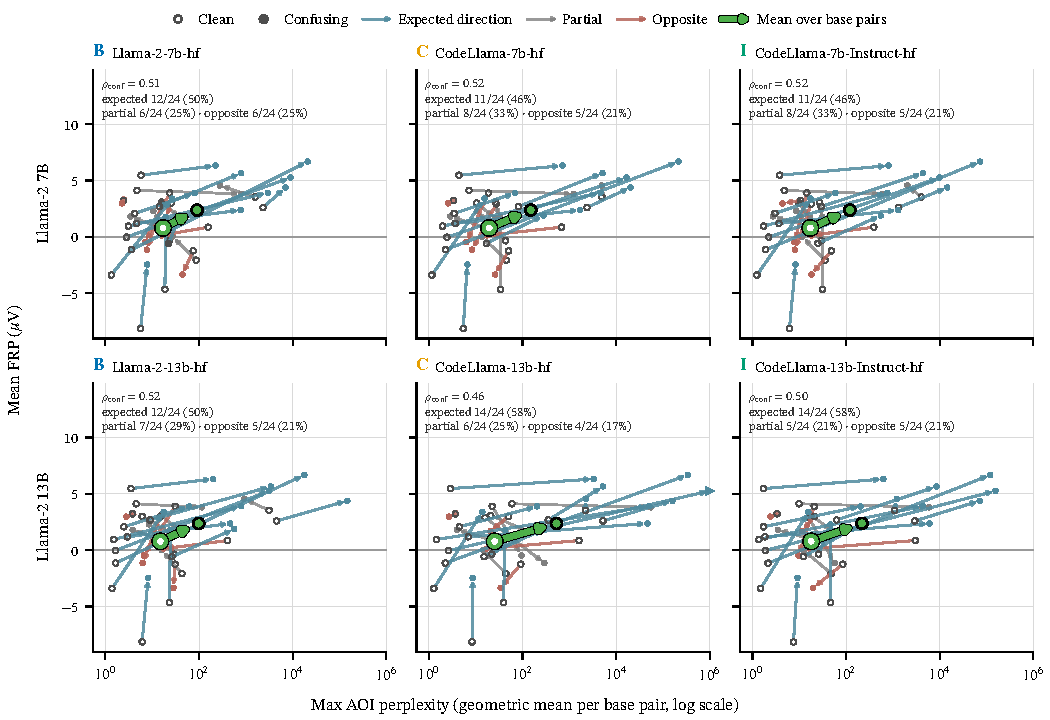
\includegraphics[width=\textwidth]{../results/extensao/2026-11-12-figuras/eeg-grade-llama2.pdf}
  \caption{Maximum AOI-level perplexity (geometric mean over the three versions of each base pair, log scale) vs.\ mean FRP for the base, code and instruct models of the Llama-2 trios (7B and 13B). Each arrow goes from the clean to the confusing version of one base pair (24 per panel), colored by direction: both perplexity and FRP increase (expected), only one increases (partial), or both decrease (opposite); the green arrow is the mean over base pairs; triangles on the right edge mark values above $10^6$. $\rho_{\mathrm{conf}}$ is the per-snippet Spearman correlation on confusing snippets (Table~\ref{tab:app-eeg}). Percentages are rounded and may not sum to 100\%.}
  \label{fig:app-eeg-llama}
\end{figure}

\begin{figure}[H]
  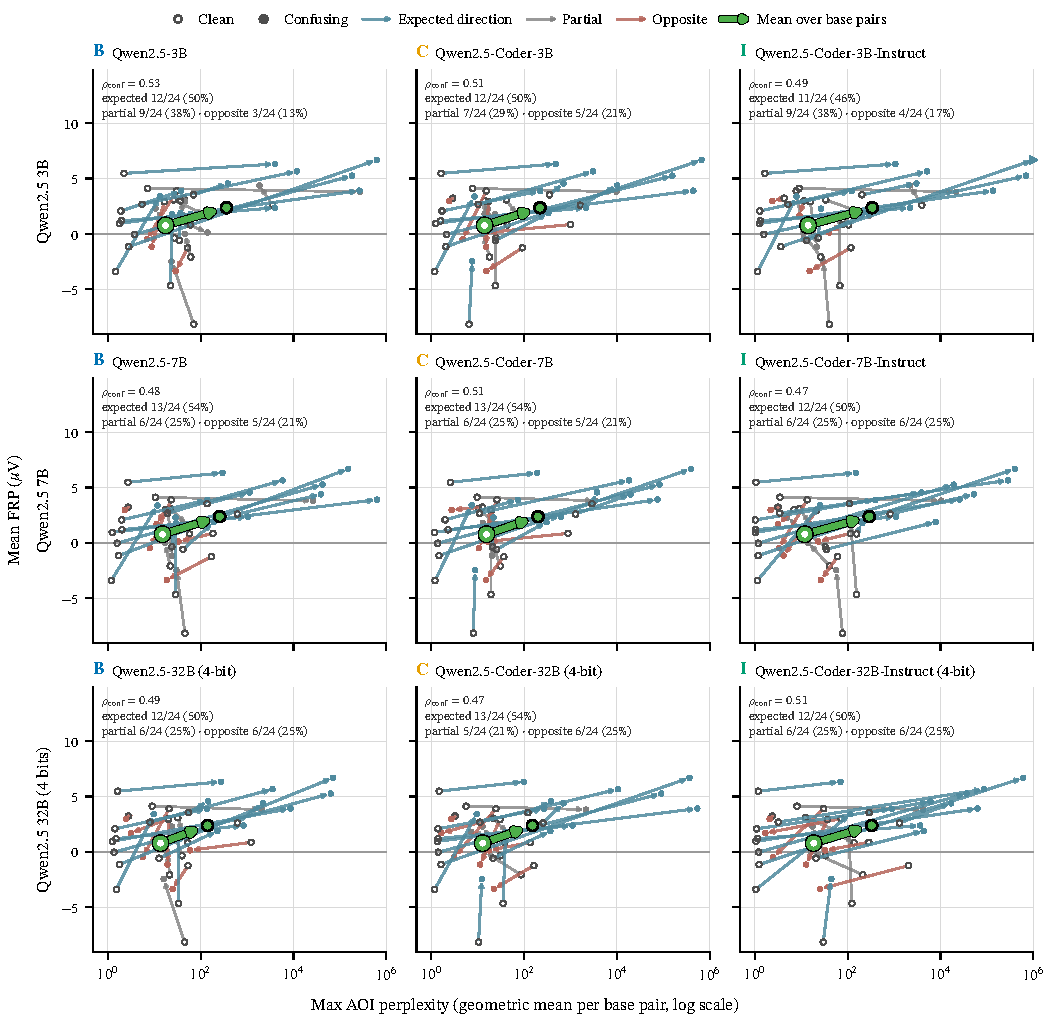
\includegraphics[width=\textwidth]{../results/extensao/2026-11-12-figuras/eeg-grade-qwen25.pdf}
  \caption{Same as Figure~\ref{fig:app-eeg-llama} for the Qwen2.5 trios (3B, 7B and 32B, the latter in 4 bits).}
  \label{fig:app-eeg-qwen}
\end{figure}


\end{document}
